\subsection{Domain Decomposition}
We implement our domain decomposition framework with flexibility in mind, in order to allow for easy experimentation, designed to integrate seamlessly with our XPINN implementation.
The computational domain, representing the physical and temporal space over which our problem is defined, is partitioned into multiple subdomains.

The subdomains themselves are composed of additive and subtractive polygons and circles, allowing for a wide variety of geometric boundaries.
The decomposition generated inherently defines the number of sub-PINNs, as well as the boundaries, meaning this does not need to be specified again later, other than loading in the generated points.
The goal of domain decomposition is, among other aspects, division of the total workload required, increasing computational efficiency.
It also offers an avenue for multiprocessing, which can quickly become cumbersome with traditional neural networks.

\subsection{Adam}
The problem at the heart of machine learning is, in effect, solving \eqref{eq:argmintheta} given a network architecture detailing the sizes and number of hidden layers and the activation functions.
This is done iteratively through the backpropagation algorithm, wherein the gradient of each layer with respect to the weights are calculated.
The weights can then be adjusted through e.g. gradient descent, with
\begin{equation}\label{eq:backprop}
    \boldsymbol{\theta}^{i+1} = \boldsymbol{\theta}^i - \gamma \frac{\partial \mathcal{C}}{\partial \boldsymbol{\theta}},
\end{equation}
where $\gamma \in \mathbb{R}_{+}$ is the step size or learning rate.

It can be shown that for small enough $\gamma$ we have $\mathcal{C}(\boldsymbol{\theta}^i) \geq \mathcal{C}(\boldsymbol{\theta}^{i+1})$, leading to convergence to a local minima.
With convex functions, this is sufficient, as a local minima is then also a global minima.
However, as permuting a layer of neurons and weights in a neural network leads to the same output, they are not convex.
A number of different optimization algorithms have been devised, often with a focus on tackling the non-convex nature of optimizing the weights of a neural network.

One such method is the Adaptive Moment Estimation (\textsc{Adam}) \cite{kingma2017adam} algorithm, which has grown incredibly popular in recent years.
The algorithm is defined by
\begin{equation}
\begin{split}
    g_{t} &\gets \nabla_{\boldsymbol{\theta}}\mathcal{C}(\boldsymbol{\theta}_t) \\
    m_{t+1} &\gets \frac{\beta_1 \cdot m_t + (1-\beta_1) \cdot g_t}{1 - \beta_1^{t+1}} \\
    v_{t+1} &\gets \frac{\beta_2 \cdot v_t + (1 - \beta_2)g_t^{\circ 2}}{1 - \beta_2^{t+1}} \\
    \boldsymbol{\theta}_{t+1}^{(n)} &\gets \boldsymbol{\theta}_t^{(n)} - \frac{\gamma}{\sqrt{\delta + v_{t+1}^{(n)}}} m_{t+1}^{(n)},
\end{split}
\end{equation}
where $m, v$ are the \nth{1} and \nth{2} moment vectors, initialized to $\boldsymbol{0}$, $\beta_1, \beta_2 \in [0,1)$ are decay rates for the moment estimates, $x^{(n)}$ denotes the $n$th component of the vector, $g^{\circ 2}$ denotes the elementwise square $g \odot g$ and $\delta > 0$ is a numerical stabilizer. 

This algorithm has effectively become the de facto standard for optimizing neural networks, however it is not without its problems.
In fact, it can fail to converge even for simple convex functions \cite{reddi2019convergence}, in contradiction to what was claimed in \cite{kingma2017adam}.
However, \textsc{Adam} has empirically performed well, which is why it grew popular in the first case.
This might have had an effect on the development of new methods within machine learning, as new methods are typically tested using \textsc{Adam} as the optimizer.
One might then question if promising methods have been discarded simply because they didn't perform well with \textsc{Adam}, as it might then have been assumed that the method itself was without merit.
However, discussing this issue in depth falls outside the scope of this paper.

Nevertheless, we utilize \textsc{Adam} in our implementation, using the \verb|Optax| \cite{deepmind2020jax} optimization library for \verb|JAX| \cite{jax2018github}.

\subsection{JAX technicalities}\label{sec:JAX}
In implementing, we focused on achieving good performance while keeping a certain degree of modularity.
This simplifies the process of changing key parameters like the subdomain decomposition, or the problem at hand.
The natural choice for implementing this was then to utilize \verb|JAX| \cite{jax2018github} within \verb|Python|.
High-Performance Computing (HPC) and Object-Oriented Programming (OOP) are two programming paradigms which are often at odds with each other, stemming from the obfuscation of the underlying computations necessary to allow for a simple interface.
We also lose out on possible problem-specific optimizations, as the program has to work in a wide variety of settings.

\verb|JAX| serves as an important component, as it allows for efficient matrix / vector operations, which are the most computationally heavy aspect of most machine learning, through just-in-time (jit) compilation.
It also implements automatic differentiation through \verb|grad|, allowing us to compute the necessary derivatives.
Note that \verb|JAX| utilizes 32-bit floating points, which give us a little over 7 digits of precision.
This limits our possible lowest loss to around $10^{-7}$, rather than the $10^{-16}$ expected with 64-bit numbers.

\subsection{Weight initialization}
We utilize a variant of Xavier initialization \cite{Glorot2010UnderstandingTD}, in order to initialize the weights of the neural networks.
For $W \in \mathbb{R}^{N_i \times N_{i-1}}$ as in \eqref{eq:A_func}, we draw
\begin{equation}
    W_{ij} \sim N\left(0, \frac{2}{N_i + N_{i-1}} \right),
\end{equation}
in order to alleviate certain issues.
If the weights are too large, errors propagate quickly through out the network, while if they are too small we run the risk of vanishing gradients.
As these issues stem from the relation between the number of neurons in a layer, and their weights, it intuitively makes sense to initialize the weights according to this relation.

It is designed to work well with $\tanh$ \cite{tanhXavier}, which is our chosen activation function for our implementation.
It is defined by
\begin{equation}
    \tanh(x) = \frac{e^x - e^{-x}}{e^x + e^{-x}},
\end{equation}
seen in \autoref{fig:tanh}.

\begin{figure}[h]
    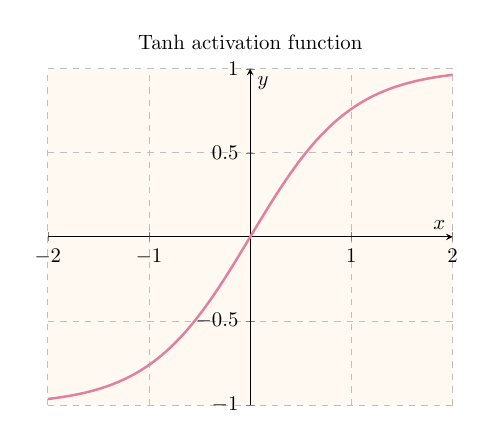
\begin{tikzpicture}[scale=0.75]
\begin{axis}[
    clip = false,
    axis lines = middle,
    xlabel = $x$,
    ylabel = $y$,
    xtick = {-2, -1, 1, 2},
    ytick = {-1, -0.5, 0.5, 1},
    ymajorgrids = true,
    xmajorgrids = true,
    grid style = dashed,
    xmin=-2, xmax=2,
    ymin=-1, ymax=1,
    title = {Tanh activation function},
    axis background/.style={fill=orange!5}
]
%Below the purple parabola is defined
\addplot [
    domain=-2:2, 
    samples=100, 
    color=purple!50,
    very thick,
]
{(e^x - e^(-x))/(e^x + e^(-x))};

\end{axis}
\end{tikzpicture}
    \caption{Tanh activation function, for $x \in [-2, 2]$.}
    \label{fig:tanh}
\end{figure}